\chapter{Richtcharakteristik kreisf"ormiger Antennen\label{chapter:kreis}}
\lhead{Richtcharakteristik kreisf"ormiger Antennen}
\begin{refsection}
\chapterauthor{Kevin Cina und Benjamin R"aber}



%Potenzreihenherleitung
\section{Potenzreihenherleitung der Besselfunktion}
Die Differenzialgleichung für die Besselfunktion lautet wiefolgt:
\begin{align}
	r^2 \cdot R''\left( r \right)
	+
	r \cdot R' \left( r \right)
	+
	\left( r^2 - n^2 \right) \cdot R \left( r \right)
	=
	0
	\label{eq:bessel_dgl}
\end{align}
Um die Differenzialgleichung zu l\"osen, w\"ahlen wir den Potenzreihenansatz mit der folgenden Potenzreihe und deren Ableitungen:
\begin{align*}
	R \left( r \right)
	&=
	r^{\sigma}
	\sum_{k=0}^{\infty} a_k \cdot r^k
\\
	R'\left( r \right)
	&=
	\sigma \cdot r^{\sigma - 1}
	\sum_{k=0}^{\infty} a_k \cdot r^k
	+
	r^{\sigma}
	\sum_{k=0}^{\infty} a_k \cdot k \cdot r^{k - 1}
\\
	R'' \left( r \right)
	&=
	\sigma \cdot \left( \sigma - 1 \right) \cdot r^{\sigma - 2}
	\sum_{k=0}^{\infty} a_k \cdot r^k
	+
	2 \cdot \sigma \cdot r^{\sigma - 1}
	\sum_{k=0}^{\infty} a_k \cdot k \cdot r^{k - 1}
	+
	r^{\sigma}
	\sum_{k=0}^{\infty} a_k \cdot k \cdot \left( k - 1 \right) \cdot r^{k - 2}	
\end{align*}
Nun kann man die Potenzreihen in die Differenzialgleichung \ref{eq:bessel_dgl} einsetzen und bekommt dann:
\begin{align*}
	\sigma \cdot \left( \sigma - 1 \right) \cdot r^{\sigma}
	\sum_{k=0}^{\infty} a_k \cdot r^k
	+
	2 \cdot \sigma \cdot r^{\sigma}
	\sum_{k=0}^{\infty} a_k \cdot k \cdot r^k
	+
	r^{\sigma}
	\sum_{k=0}^{\infty} a_k \cdot k \cdot \left( k - 1 \right) \cdot r^k
	+ \\
	\sigma \cdot r^{\sigma}
	\sum_{k=0}^{\infty} a_k \cdot r^k
	+
	r^{\sigma}
	\sum_{k=0}^{\infty} a_k \cdot k \cdot r^k
	+\\
	r^{\sigma}
	\sum_{k=0}^{\infty} a_k \cdot r^{k + 2}
	-
	n^2 \cdot r^{\sigma}
	\sum_{k=0}^{\infty} a_k \cdot r^k
	= & \text{ } 0
\end{align*}
Gleiche Summenzeichen zusammenfassen:
\begin{align*}
	\left(
	\sigma \cdot \left( \sigma - 1 \right)
	+
	\sigma
	-
	n^2
	\right)
	\cdot r^{\sigma}
	\sum_{k=0}^{\infty} a_k \cdot r^k
	+ \\
	\left(	
	2 \cdot \sigma
	+
	1
	\right)
	\cdot r^{\sigma}
	\sum_{k=0}^{\infty} a_k \cdot k \cdot r^k
	+ \\
	r^{\sigma}
	\sum_{k=0}^{\infty} a_k \cdot k \cdot \left( k - 1 \right) \cdot r^k
	+ \\
	r^{\sigma}
	\sum_{k=0}^{\infty} a_k \cdot r^{k + 2}
	= & \text{ } 0
\end{align*}
Nun muss man eine Indexgleichung für die Unbekannte $\sigma$ aufstellen, um diese zu bestimmen.
Dazu eignet sich eine Indexgleichung f\"ur den Koeffizienten $a_0$:
\begin{align*}
	\left[ \sigma \cdot \left( \sigma -1 \right) + \sigma - n^2 \right] \cdot a_0 &= 0 && \left| :a_0 \right. \\
	\sigma \cdot \left( \sigma -1 \right) + \sigma - n^2 &= 0 && \left| \text{Ausmultiplizieren} \right. \\
	\sigma ^2 - \sigma + \sigma -n^2 &= 0 && \left| \text{Vereinfachen} \right.\\
	\sigma ^2 - n^2 &= 0 && \left| +n^2 \right.\\
	\sigma ^2 &= n^2 && \left| \sqrt{\centerdot} \right. \\
	\sigma &= \pm n \text{ und } \\
	\sigma &= \pm 0 \left( \text{Doppelte Nullstelle} \right)
\end{align*}
Wir beschr\"anken uns in diesem Kapitel nur mit der L\"oesung $\sigma = \pm n$. Die L\"osung f\"ur $\sigma = \pm 0$ wird im Kapitel \nameref{chapter:thema} genauer behandelt.
Nun kann man $n$ f\"ur $\sigma$ in die Gleichung einsetzen und erh\"alt:
\begin{align*}
	\left(
	n \cdot \left( n - 1 \right)
	+
	n
	-
	n^2
	\right)
	\cdot r^{n}
	\sum_{k=0}^{\infty} a_k \cdot r^k
	+ \\
	\left(	
	2 \cdot n
	+
	1
	\right)
	\cdot r^{n}
	\sum_{k=0}^{\infty} a_k \cdot k \cdot r^k
	+ \\
	r^{n}
	\sum_{k=0}^{\infty} a_k \cdot k \cdot \left( k - 1 \right) \cdot r^k
	+ \\
	r^{n}
	\sum_{k=0}^{\infty} a_k \cdot r^{k + 2}
	= & \text{ } 0
\end{align*}
Als n\"achstes fasst man alles in eine einzige Summe zusammen und vereinfacht diese:
\begin{align*}
	r^n
	\sum_{\textcolor{red}{k=2}}^{\infty}
	\left[ n \cdot \left( n - 1 \right) \cdot a_k
	+
	2 \cdot n \cdot k \cdot a_k
	+
	k \cdot \left( k - 1 \right) \cdot a_k
	+
	n \cdot a_k
	+
	k \cdot a_k
	+
	a_{k-2}
	-
	n^2 \cdot a_k
	\right]
	\cdot r^k
	= 0 \\
	%
	r^n
	\sum_{k=2}^{\infty}
	\left[
	2 \cdot n \cdot k \cdot a_k
	+
	k^2 \cdot a_k
	+
	a_{k - 2}
	\right]
	\cdot r^k
	= 0
\end{align*}
Weil $r \neq 0$ sein muss, muss $ \left( 2 \cdot n \cdot k + k^2 \right) \cdot a_k + a_{k - 2} = 0$ sein.
Nun kann man eine Rekursion der Koeffizienten $a_k$ berechnen.
\begin{align}
	a_k
	=
	\frac
	{
		-a_{k - 2}
	}{
		k \cdot \left( 2 \cdot n + k \right)	
	}
	\label{eq:bessel_koeffreq}
\end{align}
Da $k \geq 0$ sein muss, sind nur gerade Koeffizienten m\"oglich. Somit kann man f\"ur $k$ nun $2k$ in die Gleichung \ref{eq:bessel_koeffreq} einsetzen und erh\"alt:
\begin{align*}
	a_{2k}
	&=
	\frac
	{
		-a_{2k - 2}
	}{
		2k \cdot \left( 2 \cdot n + 2k \right)	
	} \\
	&=
	\frac
	{
		-a_{2k - 2}
	}{
		4k \cdot \left( n + k \right)	
	} \\
	&=
	\frac
	{
		-a_0
	}{
		4^k \cdot {k}! \cdot {\left( n + k \right)}!
	} \\
	&=
	\frac
	{
		-a_0
	}{
		2^{2k} \cdot {k}! \cdot {\left( n + k \right)}!
	}
\end{align*}
Setzt man nun f\"ur $a_0 = \frac{1}{2^n \cdot {n}!}$ ein, so kommt man auf die Form:
\begin{align}
	J_n \left( r \right)
	&= \nonumber
	\sum_{k=0} ^{\infty}
	\frac
	{
		\left( - 1 \right) ^k \cdot r ^{2k+n}
	}{
		2^{2k+n} \cdot {k}! \cdot { \left( k + n \right) }!
	} \\
	&=
	\sum_{k=0} ^{\infty}
	\frac
	{
		\left( - 1 \right) ^k \cdot 
		\frac
		{
			r ^{2k+n}
		}{
			2^{2k+n}
		}
	}{
		{k}! \cdot { \left( k + n \right) }!
	} \\
	&=
	\sum_{k=0} ^{\infty}
	\frac
	{
		\left( - 1 \right) ^k \cdot 
		\left(		
		\frac
		{
			r
		}{
			2
		} \right) ^{2k+n}
	}{
		{k}! \cdot { \left( k + n \right) }!
	}
	\label{eq:bessel_summenformel}
\end{align}

\begin{figure}
	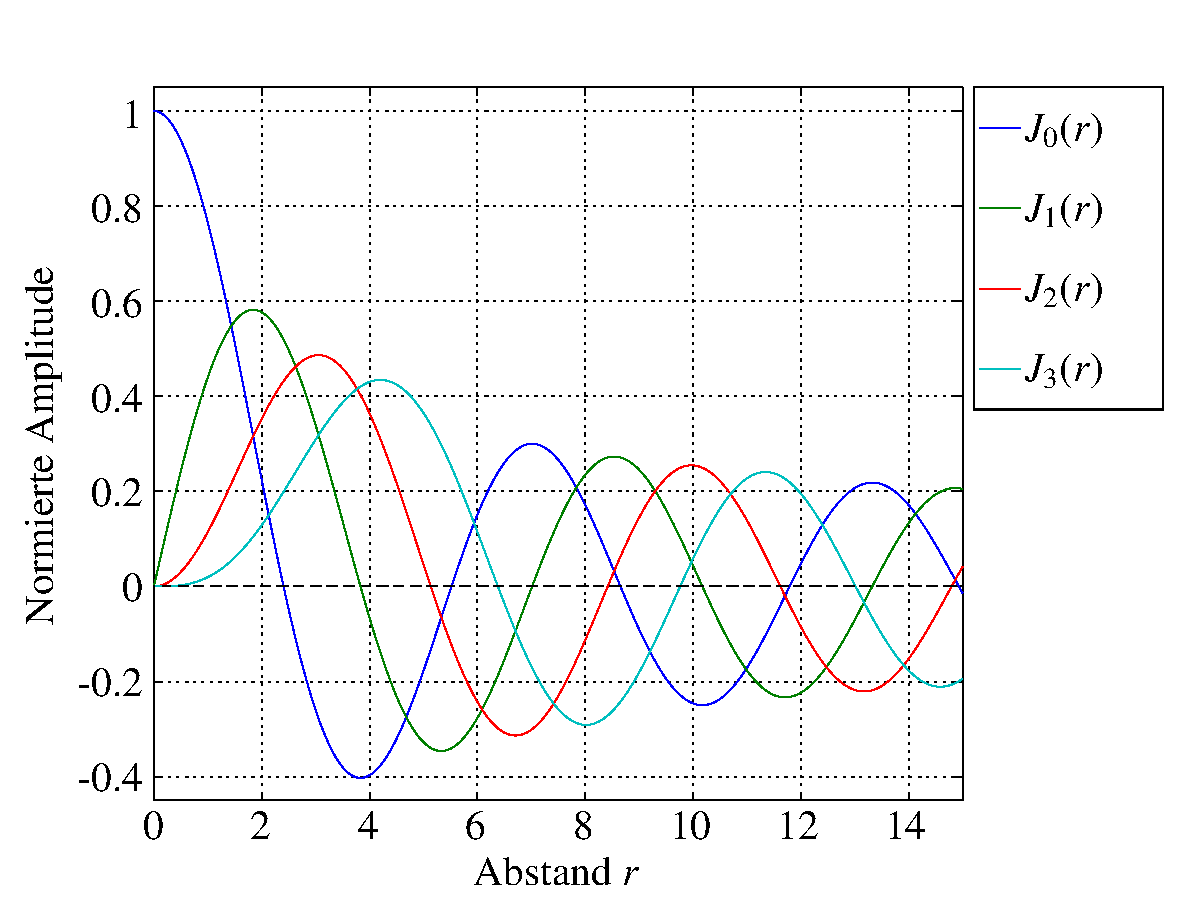
\includegraphics[scale=0.75]{kreis/besselfunction.png}
	\label{img:besselfunction}
	\caption[Besselfunktion]{Besselfunktion geplottet}
\end{figure}

\printbibliography[heading=subbibliography]
\end{refsection}

